\documentclass{beamer}

\title{The Impact of Anthropogenic Forcing on ENSO Amplitude}
\author{Ben Goldman}
\date{\today}

\usepackage{natbib}
\usepackage{tikz}
\usepackage{varwidth}

\usetheme{ben}
\setbeamersize{description width=0.5cm}

\usetikzlibrary{arrows,snakes,backgrounds}
\tikzstyle{process}=[rectangle, draw=process, fill=process!20, line width = 0.3mm]
\tikzstyle{data}=[rectangle, draw=data, fill=data!20, line width = 0.3mm]
\tikzstyle{tight}=[node distance = 0.5in]
\tikzstyle{loose}=[node distance = 2in]
\definecolor{process}{HTML}{3d5f8f}
\definecolor{data}{HTML}{8f6d3d}

\newcommand{\myfig}[3]{
  \begin{figure}
    \centering
    \includegraphics[width=\textwidth]{figures/#1}
    \caption{#2}
    \label{fig:#3}
  \end{figure}
}
\renewcommand{\bibsection}{}


\begin{document}

\maketitle

\section{Introduction}

\begin{frame}{Climate Change and Variability}
  \begin{columns}
    \column{0.4\textwidth}
    \begin{itemize}
    \item Global warming
    \item Long-term trends vs short-term randomness
    \end{itemize}
    \column{0.6\textwidth}
    \myfig{intro_fig_3.pdf}{Global mean land air temperature in GISSTEMP 4 dataset. \citep{gistemp2019giss} and \citep{lenssen2019improvements}}{this}
  \end{columns}
\end{frame}

\begin{frame}{Climate forcing}
  \begin{columns}
    \column{0.5\textwidth}
    \begin{itemize}
    \item \alert{Forcing}: any external factor that affects climate.
      \begin{description}
      \item[\alert{GHG}] Greenhouse gasses
      \item[\alert{AER}] Aerosols (natural: volcanic ash, artificial: smoke)
      \item[\alert{BMB}] Biomass burning
      \item[\alert{LULC}] Land use/cover (deforestation, desertification)
      \end{description}
    \end{itemize}
    \column{0.6\textwidth}
    \myfig{greenhouse_Effect.jpg}{Factors that contribute to the greenhouse effect.}{this}
  \end{columns}
\end{frame}

\begin{frame}{El Niño (ENSO)}
  \begin{figure}
    \begin{columns}
      \column{0.5\textwidth}
      \begin{itemize}
      \item Warming and cooling of the Pacific Ocean.
      \item Affects human societies through temperature and rainfall. \citep{ropelewski1987global}
      \item May be affected by climate change.
      \end{itemize}
      \caption{Comparison of SST anomaly between 1975 La Niña event and 1997 El Niño event in HadISST 1 dataset. \citep{rayner2003global}}
      \column{0.5\textwidth}
      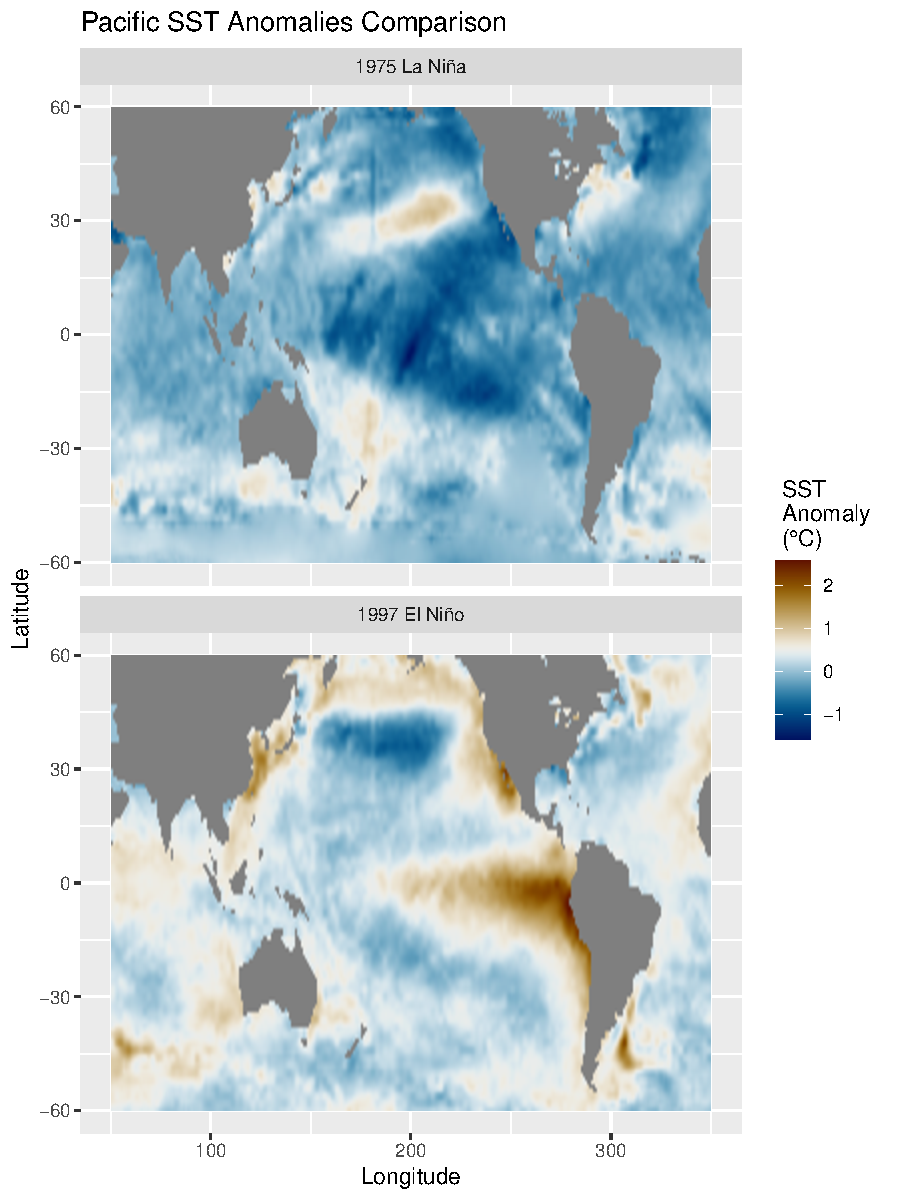
\includegraphics[width = \textwidth]{figures/intro_fig.pdf}
    \end{columns}
  \end{figure}
\end{frame}

\begin{frame}{Method: Climate Simulation}
  \begin{itemize}
  \item Run climate simulation with predicted forcing levels as input.
  \item \alert{Ensemble:} set of repeated simulations of the same model.
  \end{itemize}
  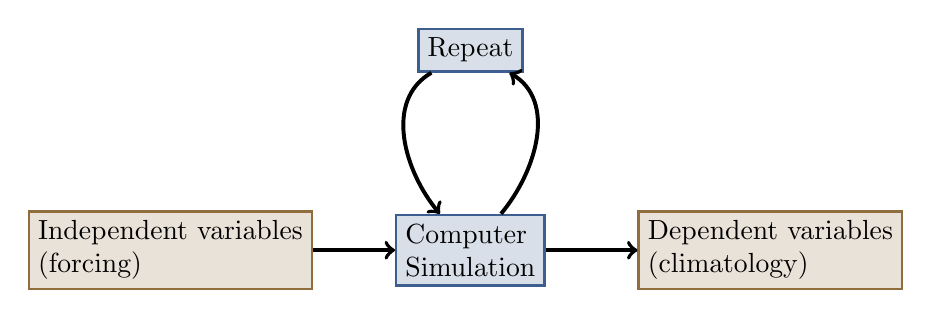
\begin{tikzpicture}[node distance = 1.5in, line width = 0.5mm]
    \node (input) [data] {
      \begin{varwidth}{1.5in}
        Independent variables (forcing)
      \end{varwidth}};
    \node (model) [right of=input] [process] {
      \begin{varwidth}{\linewidth}
        Computer\\Simulation
      \end{varwidth}};
    \node (output) [right of=model] [data] {
      \begin{varwidth}{1.4in}
        Dependent variables (climatology)
      \end{varwidth}};
    \node (repeat) [above of=model, node distance = 1in] [process] {
      \begin{varwidth}{0.5in}
        Repeat
      \end{varwidth}};
    \draw [->] (input) to (model);
    \draw [->] (model) to (output);
    \draw [->] (model) to [out = 50, in = 330] (repeat);
    \draw [->] (repeat) to [out = 210, in = 130] (model);
  \end{tikzpicture}
\end{frame}

\begin{frame}{Review of Literature}
  \begin{itemize}
  \item ENSO's properties observed vary across different decades. \citep{lubbecke2014assessing}.
  \item ENSO responds to external forcing.
    \begin{itemize}
    \item Correlation between ENSO strength and sunspot activity \citep{emile2007nino}.
    \item Weakened ENSO during the Ice Age due to reduced CO$_2$ levels \citep{zhu2017reduced}.
    \end{itemize}
  \item Models show possible increasing ENSO activity in the future \citep{zheng2017response} and \citep{maher2018enso}.
  \item Factors other than CO$_2$ can affect ENSO.
    \begin{itemize}
    \item Ozone emissions reduce ENSO activity \citep{nowack2017role}.
    \item Aerosol emissions modify ENSO geographical center \citep{stevenson2017forced}.
    \end{itemize}
  \end{itemize}
\end{frame}

\begin{frame}{Gap}
  \begin{itemize}
  \item Little research using a large ensemble to examine the effect of individual factors on ENSO.
  \item Considerable disagreement between studies on whether ENSO will strengthen or weaken due to global warming
  \end{itemize}
\end{frame}

\begin{frame}{Questions}
  \begin{description}
  \item[What?] Do the CESM1 and CESM2 predict increased or decreased ENSO intensity in the future?
  \item[Why?] Is the predicted increase (or decrease) due to human activities?
  \item[How?] What processes are causing greenhouse gasses and aerosols to affect ENSO?
  \end{description}
\end{frame}

\section{Data, Methods, and Results}

\begin{frame}{Methods Overview}
  \begin{itemize}
  \item Precollected predictions of sea surface temperature from climate models.
  \item Calculate ENSO intensity in model output.
  \item Use single forcing ensembles to estimate contributions each forcing item.
  \item Plot correlation between ENSO intensity and ocean temperature to examine relationship between heat transfer, forcing, and ENSO.
  \item Use wavelet analysis to analyze changes to ENSO at different frequencies.
  \end{itemize}
\end{frame}

\begin{frame}{Role of Mentor and Student}
  \begin{columns}[t]
    \column{.5\textwidth}
    Student:
    \begin{itemize}
    \item Analyze raw data on computer
    \item Produce graphics for analysis and publication
    \item Write documentation
    \item Identify key features of results
    \end{itemize}
    \column{.5\textwidth}
    Mentor:
    \begin{itemize}
    \item Review student writing
    \item Interpret results in the context of climatology
    \item Conduct parallel analysis
    \item Provide raw data from facility
    \end{itemize}
  \end{columns}

\end{frame}

\begin{frame}{Model Setup}
  \begin{itemize}
  \item CESM1 \citep{kay2015community} and CESM2 \citep{danabasoglu2020community}
  \item Observed forcing levels from 1850-2005
  \item Predicted forcing levels from 2005-2100
  \item Ensembles have 40 and 50 simulations respectively
  \item Control simulation with pre-1850 forcing levels
  \item Single forcing ensembles that represent influence of single factor
  \end{itemize}
\end{frame}

\begin{frame}{Measuring ENSO Intensity}
  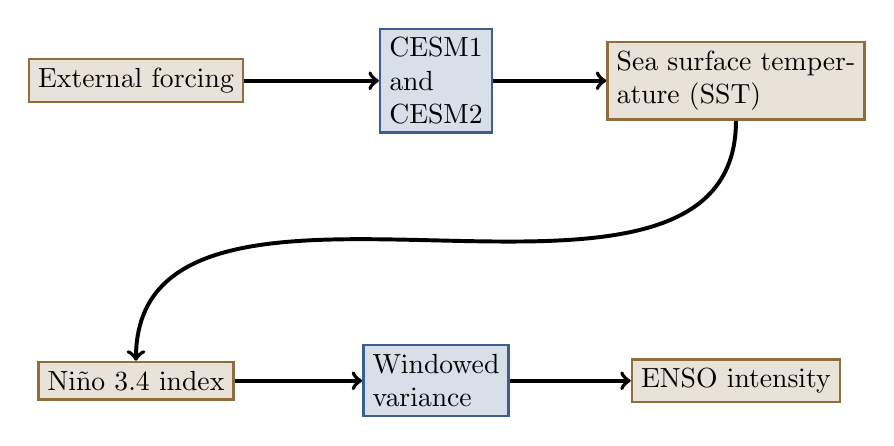
\begin{tikzpicture}[node distance = 1.5in, line width = 0.5mm]
    \node [data] (input) {
      \begin{varwidth}{1.5in}
        External forcing
      \end{varwidth}};
    \node [process] (model) [right of=input] {
      \begin{varwidth}{\linewidth}
        CESM1\\and\\CESM2
      \end{varwidth}};
    \node [data] (output) [right of=model] {
      \begin{varwidth}{1.2in}
        Sea surface temperature (SST)
      \end{varwidth}};
    \node [data] (nino) [below of=input] {
      \begin{varwidth}{1.4in}
        Niño 3.4 index
      \end{varwidth}};
    \node [process] (variance) [right of=nino] {
      \begin{varwidth}{1.4in}
        Windowed\\variance
      \end{varwidth}};
    \node [data] (intensity) [right of=variance] {
      \begin{varwidth}{1.4in}
        ENSO intensity
      \end{varwidth}};
    \draw [->] (input) to (model);
    \draw [->] (model) to (output);
    \draw [->] (output) to [out = 270, in = 90] (nino);
    \draw [->] (nino) to (variance);
    \draw [->] (variance) to (intensity);
  \end{tikzpicture}
\end{frame}

\begin{frame}{ENSO is Becoming Stronger}
  \begin{columns}
    \column{0.5\textwidth}
    \begin{itemize}
    \item Increase in ENSO intensity in both ensembles.
    \item Increase slows down in CESM1 and decreases in CESM2 after around 2050.
      \begin{itemize}
      \item May be caused by aerosol emissions.
      \end{itemize}
    \end{itemize}
    \column{0.5\textwidth}
    \myfig{ff_compare.pdf}{ENSO intensity ensemble mean and standard error for CESM1 and CESM2}{ff_compare}
  \end{columns}
\end{frame}

\begin{frame}{Influence of Aerosols and Greenhouse Gasses}
  \begin{columns}
    \column{0.65\textwidth}
    \begin{itemize}
    \item Influence of each factor on ENSO amplitude.
    \item Increased variance due to greenhouse gas emissions.
    \item Somewhat increased variance from aerosol emissions, but not linear.
    \item Inconclusive results from biomass burning and land use forcing
    \end{itemize}
    \alert{Takeaway:} Human activities are triggering predicted strengthening of ENSO.
    \column{0.5\textwidth}
    \myfig{cesm1_sf.pdf}{Influence of GHG, AER, and BMB forcing on ENSO amplitude in CESM1}{cesm1_sf}
  \end{columns}
\end{frame}

\begin{frame}{Correlation With Ocean Temperature}
  \begin{columns}
    \column{0.65\textwidth}
    \begin{itemize}
    \item Correlation coefficient between ocean temperature and ENSO amplitude.
    \item Negative coefficient in subsurface layer.
    \item Positive coefficient in surface layer.
    \item Suggests that ocean stratification may be mediating global warming influence on ENSO.
    \item Difference in heating modifies mechanics of ENSO cycle.
    \end{itemize}
    \column{0.5\textwidth}
    \myfig{tempdt.pdf}{Correlation coefficient between ENSO amplitude and ocean temperature in equatorial cross-section in the fully-forced CESM1 ensemble}{tempdt}
  \end{columns}
\end{frame}

\begin{frame}{Wavelet Analysis}
  \begin{columns}
    \column{0.6\textwidth}
    \begin{itemize}
    \item Separate ENSO record into frequency over time.
    \item Increase in power in late 21\textsuperscript{st} century agrees with previous results.
    \item CESM2 shows a slight ``speeding up'' of ENSO as period decreases in late 21\textsuperscript{st} century.
    \end{itemize}
    \column{0.6\textwidth}
    \myfig{wavelet2.pdf}{Wavelet power spectrum for the Niño 3.4 index in the fully-forced CESM1 and CESM2 ensembles}{wavelet2}
  \end{columns}
\end{frame}

\section{Conclusion}

\begin{frame}{Conclusions and Discussion}
  \begin{itemize}
  \item There is likely to be an increase in ENSO strength over the next 100 years. Agrees with \citet{cai2018increased}.
  \item Variance increase is likely caused by the combined influence of greenhouse gasses and aerosols.
  \item Global warming increases ENSO intensity by warming upper layers of the Pacific faster than central layers.
  \end{itemize}
\end{frame}

\begin{frame}{Application, Limitation, and Next Steps}
  \begin{description}
  \item[\alert{Application}] Improve prediction ability to help people prepare for increased likelihood of extreme weather.
  \item[\alert{Limitation}] Niño 3.4 index may not be fully accurate for various models \citep{cai2018increased}. Also, CESM may contain biases and is not completely accurate.
  \item[\alert{Next steps}] Examine other variables to further analyze mediator process, continue wavelet analysis methods to focus on individual frequency bands.
  \end{description}
\end{frame}

\begin{frame}{Acknowledgments}
  \begin{itemize}
  \item This material is based upon work supported by the National Center for Atmospheric Research, which is a major facility sponsored by the National Science Foundation under Cooperative Agreement No. 1852977.
  \item Thank you to my teacher, my family, and my mentor!
  \item Software used: R, ncdf4, zoo, dplyr, ggplot2, WaveletComp, reshape2, nco.
  \end{itemize}
\end{frame}

\begin{frame}{References}
  \bibliographystyle{apalike}
  \fontsize{4pt}{5}\selectfont
  \bibliography{references.bib}
\end{frame}

\end{document}





% hi
